\chapter{Resultados}




\section{Sistema de cifrado}

\subsection{Inversión de Bits}


Una vez que el sistema de cifrado recibe un paquete RTP, se dealiza uno  de los pasos que conforman el algoritmo propuesto:  diffuse and destroy the meaning of compressed codeword sequence and meke it impractial to predict the original codeword sequence. Para lograr esto, se propone la inversión da al menos un bit cada  $BF = F \cdot Av \cdot MEPS$ bits, donde $Av$ es el tamaño promedio de los códigos de Huffman, MEPL is the calculated Mean Average Propagation Length (MEPL) in codeword units, $Av \cdot MEPL$ es el promedio del error de propagación en bits, y $f$ is a tunable security factor with values $ \frac{1}{MEPL}  \leq f \leq \frac{3}{4}$. Para este rango de $f$, $Av \leq BF \leq Av \cdot MEPL$ esto es, al menos un bit es invertido per average Huffman codeword size ($Av$) up to $\frac{3}{4}(Av \cdot MEPL)$ bits. Esto es lo que hace nuestro system scalable secured, as $f$ gets smaller more bits are flipoed per  $BF$-bits units increasing de system security. Depending of the specific needs of the user, $f$ provides a tradeoff between security and performance.

The actual locariton $B_{i}$ del bit a ser invertido en el flujo es calculado como sigue:

\begin{equation}
B_{i}= \left( rand   \lceil \log_{2}(f \cdot Av \cdot MEPL)  \rceil \mod{BF}      \right) +1
\end{equation}

donde $rand(Numero_bits)$ is our own designed PRNG function describes in the previous section. EL argumento $ \lceil \log_{2}(f \cdot Av \cdot MEPL)  \rceil$ representa la longitud de bits of the requested random number with límites $1 \leq B_{i} \leq BF$.

The algoritm for random bit flipping in the payload P of size $P_{s}$ bytes es outlined in the following:

PONGO ALGORITMO CON LA LIBRERIA ALGORITM2e

\subsection{Segment shuffling}

Después de que ha crecido el  proceso de inversión de bits, ahora, es necesario permutar los RTP-packet payload by performing an L-way shuffling. Here the payload is divided into L segmentes which are schuffled using the algorithm described below and ilustrate in figure ~\ref{shuffling}

\begin{figure}[H]
\centering
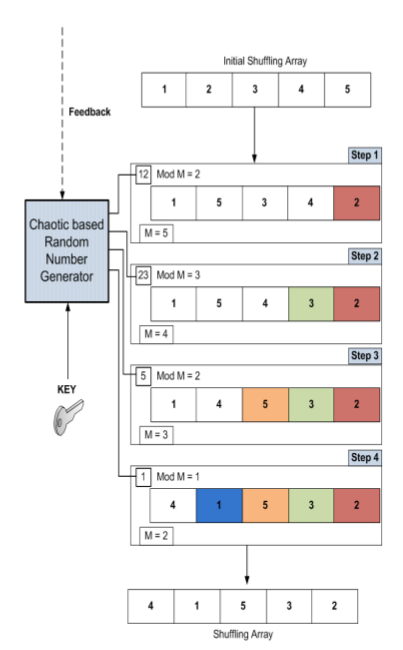
\includegraphics[width=7cm]{logos/per.png}
\caption{Esquema de permutacion.}
\label{shuffling}
\end{figure}



